\section{Tổng kết}
\subsection{Kết quả giai đoạn 1}
Sau khi kết thúc giai đoạn 1, nhóm chúng em đã xác định được phạm vi cũng như các yêu cầu cần thiết của hệ thống. Hệ thống được thiết kế hướng đến việc nâng cao trải nghiệm học tập và tạo động lực học toán cho học sinh tiểu học thông qua các tính năng tương tác, game hóa và theo dõi tiến độ học tập chi tiết.

\newline
\vspace{0.2cm}
Sau khi kết thúc giai đoạn 1, nhóm đã hoàn thành được các công việc sau đây:
\begin{enumerate}
	\item Xác định được phạm vi và yêu cầu của hệ thống cho phù hợp với nhu cầu sử dụng của người dùng hiện tại, cụ thể là học sinh ở cấp bậc Tiểu học và phụ huynh có con em đang học tập tại cấp bậc này. 
	\item Thiết kế được cơ sở dữ liệu để đáp ứng được các yêu cầu lưu trữ của hệ thống.
	\item Thiết kế giao diện người dùng trên nền tảng web và đặt ra các tiêu chí để đánh giá giao diện, bao gồm: thân thiện với người dùng, sáng tạo, độc đáo, thu hút người dùng và đáp ứng được các yêu cầu nghiệp vụ của hệ thống. Các giao diện bao gồm:
	\begin{itemize}
		\item \textbf{Đối với học sinh:} Trang chủ, trang bài học, trang chủ đề, trang đấu trường, trang bài tập, trang bài thi, trang xếp hạng, trang nhiệm vụ, trang minigames, trang lịch sử làm bài, giao diện quản lý tài khoản cá nhân bao gồm cập nhật thông tin cá nhân (ảnh đại diện, tên, lớp), đổi mật khẩu, liên kết tài khoản. 
		\item \textbf{Đối với phụ huynh:} Trang chủ, trang thống kê tổng quan, trang lịch sử làm bài, trang minigames, giao diện quản lý tài khoản cá nhân bao gồm cập nhật thông tin cá nhân (ảnh đại diện, lớp), đổi mật khẩu, liên kết tài khoản, nâng cấp tài khoản.
	\end{itemize}
	\item Thiết kế và hiện thực được một số dạng bài tập tương tác (mục \ref{subsec:interact}).
	\item Hiện thực được 1 minigame là Math Match.
	\item Hiện thực được các API cơ bản: 
	\begin{itemize}
		\item Đăng nhập, đăng ký tài khoản.
		\item Quản lý hồ sơ người dùng (xem và cập nhật thông tin cá nhân).
		\item Cập nhật tiến độ học tập.
		\item Cập nhật điểm tích tích lũy (thạch anh) cho người dùng.
		\item Lấy các dữ liệu về khối lớp, thế giới và các vùng đất liên quan, chủ đề, bài học, bài tập dạng tương tác.
	\end{itemize}
	\item Hiện thực được các logic ở frontend như sau:
	\begin{itemize}
		\item Đăng nhập, đăng ký tài khoản.
		\item Cập nhật thông tin học sinh trên trang Onboarding (mục \ref{subsec:onboarding}), nâng cao sự gắn kết giữa người dùng và hệ thống.
		\item Cập nhật thông tin người dùng (ảnh đại diện, họ và tên, khối lớp).
		\item Tích hợp được các dạng bài tập tương tác vào giao diện, đồng thời hoàn thành luồng làm bài tập cơ bản bao gồm: 
		\newline 
		Chọn lớp $\rightarrow$ Chọn chủ đề $\rightarrow$ Chọn bài học Làm bài $\rightarrow$ Xem kết quả
	\end{itemize}
\end{enumerate}

\subsection{Kế hoạch và phân công công việc giai đoạn 1}

\renewcommand{\arraystretch}{1.3}

\begin{longtable}{|>{\centering\arraybackslash}m{1.5cm}|m{7cm}|m{5cm}|}
	\hline
	\textbf{Tuần} & \textbf{Công việc} & \textbf{Người thực hiện} \\
	\hline
	\endfirsthead
	
	\hline
	\textbf{Tuần} & \textbf{Công việc} & \textbf{Người thực hiện} \\
	\hline
	\endhead
	
	\hline
	\endfoot
	
	38-39 & Xác định phạm vi đề tài: xây dựng website học toán tư duy cho học sinh tiểu học & Nguyễn Văn Thành \\
	\cline{2-3}
	& Xác định đối tượng người dùng, stakeholders và hệ thống liên quan & Trương Anh Khoa \\
	\cline{2-3}
	& Thống nhất yêu cầu người dùng và các chức năng cần thiết & Nguyễn Văn Thành, \newline Nguyễn Minh Tân, \newline Trương Anh Khoa \\
	\cline{2-3}
	& Thiết kế giao diện người dùng: Trang Landing, Trang chủ (học sinh), Trang Bài học và giao diện popup quản lý tài khoản người dùng. & Nguyễn Minh Tân \\
	\hline
	
	40-41 & Vẽ usecase diagram cho toàn bộ hệ thống và activity diagram cho các luồng Đăng nhập, Đăng ký, Làm bài tập. & Trương Anh Khoa \\
	\cline{2-3}
	& Vẽ sequence diagram cho các luồng Đăng nhập, Đăng ký, Làm bài tập. & Nguyễn Minh Tân \\
	\cline{2-3}
	& Thiết kế cơ sở dữ liệu. & Nguyễn Văn Thành \\
	\cline{2-3}
	& Thiết kế giao diện người dùng: Trang Milestone, Trang Đấu trường, Bảng xếp hạng, Trang Nhiệm vụ, Trang Làm bài kiểm tra. & Nguyễn Minh Tân \\
	\hline
	
	42-43 & Thiết kế kiến trúc hệ thống (Frontend – Backend – Database) & Nguyễn Văn Thành \\
	\cline{2-3}
	& Tạo các repository để quản lý mã nguồn cho frontend và backend & Nguyễn Văn Thành, \newline Nguyễn Minh Tân, \newline Trương Anh Khoa \\
	\cline{2-3}
	& Thiết kế giao diện người dùng: Trang Minigame, Trang Thống kê (phụ huynh), Trang Lịch sử làm bài & Nguyễn Minh Tân \\
	\hline
	
	44-45 & Setup backend, cấu hình server, tạo database và các bảng chính & Nguyễn Văn Thành \\
	\cline{2-3}
	& Hiện thực giao diện người dùng: Trang Landing, Trang chủ (học sinh), Trang Đấu trường, Trang Đăng nhập/Đăng ký, Trang Onboarding, Trang Milestone, Trang Lấy lại mật khẩu. & Nguyễn Minh Tân \\
	\cline{2-3}
	& Hiện thực giao diện người dùng: Trang Bài học, Trang Nhiệm vụ, Trang Bảng xếp hạng, giao diện quản lý tài khoản người dùng bao gồm Chỉnh sửa thông tin cá nhân, Đổi mật khẩu, Liên kết tài khoản. & Trương Anh Khoa \\
	\cline{2-3}
	& Hiện thực các API đăng nhập, đăng ký, lấy danh sách các chủ đề theo lớp. & Nguyễn Văn Thành \\
	\hline
	
	46-47 & Thiết kế các dạng bài tập tương tác (nối, đúng/sai, tô màu, kéo thả, điền khuyết) & Trương Anh Khoa \\
	\cline{2-3}
	& Hiện thực các dạng bài tập tương tác. & Trương Anh Khoa \\
	\cline{2-3}
	& Hoàn thiện và nối API cho chức năng đăng nhập và đăng ký tài khoản. & Nguyễn Minh Tân \\
	\cline{2-3}
	& Hiện thực các API quản lý khối lớp, chủ đề, bài tập, cập nhật điểm, quản lý tiến trình học tập & Nguyễn Văn Thành \\
	\hline
	
	48-49 & Hoàn thiện luồng làm bài tập tương tác ở frontend. & Nguyễn Minh Tân, \newline Trương Anh Khoa \\
	\cline{2-3}
	& Thiết kế và hoàn thiện minigame Math Match. & Trương Anh Khoa \\
	\cline{2-3}
	& Hiện thực các API quản lý tài khoản người dùng, gợi ý chủ đề học tập theo thời gian, quản lý đấu trường & Nguyễn Văn Thành \\
	\hline
	
	50-51 & Tối ưu backend, fix bugs, refactor code & Nguyễn Văn Thành \\
	\cline{2-3}
	& Hoàn thiện và nối API cho các chức năng quản lý tài khoản người dùng & Trương Anh Khoa \\
	\cline{2-3}
	& Hoàn thiện và nối API cho các chức năng chơi minigame, hiển thị tiến trình học tập & Nguyễn Minh Tân \\
	\cline{2-3}
	& Kiểm tra lại các chức năng cơ bản đã được hiện thực & Nguyễn Văn Thành, \newline Nguyễn Minh Tân, \newline Trương Anh Khoa \\
	\hline
	
\end{longtable}

\begin{figure}[H]
	\centering
	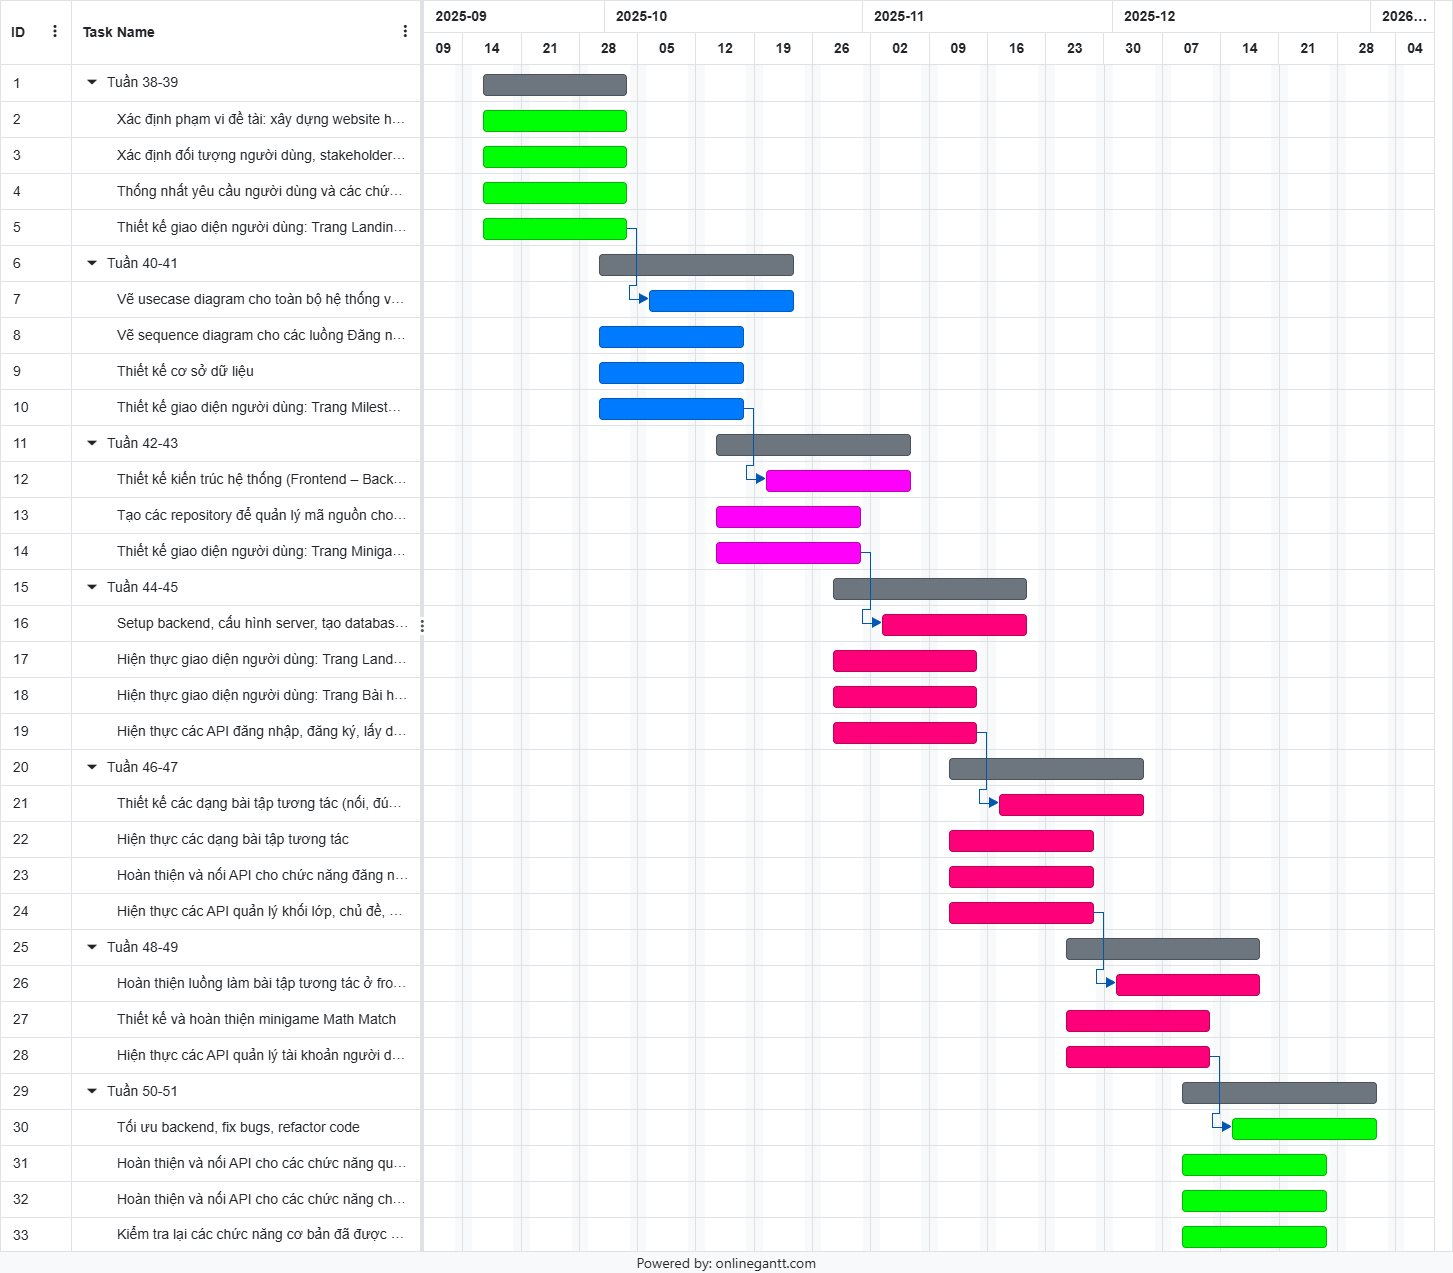
\includegraphics[width=\textwidth]{Image/phase1.jpg}
	\vspace{0.5cm}
	\caption{Biểu đồ Gantt giai đoạn 1}
	\label{fig:gantt-phase1}
\end{figure}


\newpage
\subsection{Kế hoạch và phân công công việc giai đoạn 2}
\renewcommand{\arraystretch}{1.3}
\begin{longtable}{|>{\centering\arraybackslash}m{2cm}|p{7.5cm}|p{4.5cm}|}
	\hline
	\textbf{Tuần} & \textbf{Công việc (Chi tiết thực hiện)} & \textbf{Người thực hiện} \\
	\hline
	\endfirsthead
	
	\hline
	\textbf{Tuần} & \textbf{Công việc (Chi tiết thực hiện)} & \textbf{Người thực hiện} \\
	\hline
	\endhead
	
	\hline
	\endfoot
	
	Tuần 1--2 & \textbf{Khởi động \& Triển khai tính năng Assessment cơ bản:} 
	
	\textbullet\ \textbf{BE:} Thiết kế cấu trúc cơ sở dữ liệu (Schema) cho Assessment, AssessmentResult và Answer. Xây dựng hệ thống API CRUD hoàn chỉnh để tạo, liệt kê và xem chi tiết bài kiểm tra. Thiết lập môi trường Swagger và chuẩn bị dữ liệu mẫu (Seed data). 
	
	\textbullet\ \textbf{FE:} Xây dựng giao diện danh sách các bài kiểm tra hiện có. Thiết kế trang chi tiết bài kiểm tra bao gồm mô tả, yêu cầu và thông tin tổng quan. Kết nối dữ liệu từ API để hiển thị lên giao diện. Hiện thực logic nghiệp vụ cho tính năng Đấu trường.
	
	\textbullet\ \textbf{Game:} Nghiên cứu và thiết kế bộ bài tập bám sát chương trình học của bộ Giáo dục và Đào tạo. & BE: Nguyễn Văn Thành
	
	FE: Nguyễn Minh Tân
	
	Game: Trương Anh Khoa \\
	\hline
	
	Tuần 3--4 & \textbf{Nộp bài \& Quy trình chấm điểm tự động:} 
	
	\textbullet\ \textbf{BE:} Hoàn thiện logic xử lý khi người dùng nộp bài (POST /submit). Xây dựng bộ máy chấm điểm tự động (Auto-grading) cho trắc nghiệm và đúng/sai. Viết unit test và tích hợp để kiểm tra luồng dữ liệu từ lúc nộp đến khi lưu điểm. 
	
	\textbullet\ \textbf{FE:} Phát triển giao diện làm bài trực tuyến (Quiz Interface). Tích hợp logic bộ đếm ngược thời gian và trình quản lý trạng thái câu trả lời (State Management). Xây dựng màn hình hiển thị kết quả bài thi ngay sau khi nộp. 
	
	\textbullet\ \textbf{Game:} Nghiên cứu các dạng bài tập tương tác. Thiết kế các assets và hiệu ứng hình ảnh tương ứng. & BE: Nguyễn Văn Thành
	
	FE: Nguyễn Minh Tân
	
	Game: Trương Anh Khoa \\
	\hline
	
	Tuần 5--6 & \textbf{Mission \& Achievement (Nhiệm vụ \& Thành tựu):} 
	
	\textbullet\ \textbf{BE:} Thiết kế Model Mission và Achievement. Xây dựng logic tự động cập nhật tiến trình (Progress) dựa trên hành động của người dùng (ví dụ: hoàn thành bài học, đăng nhập hàng ngày). API quản lý danh sách thành tựu người dùng đạt được. 
	
	\textbullet\ \textbf{FE:} Xây dựng Dashboard nhiệm vụ tập trung. Hiển thị danh sách nhiệm vụ hàng ngày/tuần kèm thanh tiến trình trực quan. Thiết kế trang hồ sơ cá nhân hiển thị kho huy hiệu thành tựu. 
	
	\textbullet\ \textbf{Game:} Xây dựng tính năng xem trước câu hỏi bài tập cho admin. & BE: Nguyễn Văn Thành
	
	FE: Nguyễn Minh Tân
	
	Game: Trương Anh Khoa \\
	\hline
	
	Tuần 7--8 & \textbf{RewardRecord \& Cơ chế thưởng:} 
	
	\textbullet\ \textbf{BE:} Triển khai Model RewardRecord để quản lý lịch sử biến động phần thưởng (Quartz, BP). Đảm bảo tính atomicity (giao dịch an toàn) khi cộng thưởng vào ví người dùng. Xác thực nguồn gốc phần thưởng để tránh lỗi dữ liệu. 
	
	\textbullet\ \textbf{FE:} Xây dựng giao diện admin quản lý người dùng, bao gồm danh sách tài khoản, chức năng tìm kiếm, lọc theo vai trò và khóa/mở khóa tài khoản. Thiết kế trang thống kê tổng quan cho admin.
	
	\textbullet\ \textbf{Game:} Nghiên cứu minigame tương tác 2 người thông qua server. & BE: Nguyễn Văn Thành
	
	FE: Nguyễn Minh Tân
	
	Game: Trương Anh Khoa \\
	\hline
	
	Tuần 9--10 & \textbf{FamilyGame \& FamilyReport (Tính năng gia đình):} 
	
	\textbullet\ \textbf{BE:} Xây dựng logic cho FamilyGame và tham gia nhóm. Thiết lập thuật toán tổng hợp dữ liệu để sinh báo cáo gia đình (FamilyReport), tính toán hiệu suất học tập trung bình của cả nhóm. 
	
	\textbullet\ \textbf{FE:} Thiết kế giao diện báo cáo gia đình với các biểu đồ so sánh (sử dụng thư viện biểu đồ). Xây dựng sảnh chờ (Lobby) cho các thành viên gia đình tương tác. 
	
	\textbullet\ \textbf{Game:} Phát triển logic và giao diện cho mini-game thi đấu giữa các thành viên. Đảm bảo tính đồng bộ dữ liệu điểm số trong thời gian thực. & BE: Nguyễn Văn Thành
	
	FE: Nguyễn Minh Tân
	
	Game: Trương Anh Khoa \\
	\hline
	
	Tuần 11--12 & \textbf{LectureResult \& ExerciseResult (Lưu trữ chi tiết):} 
	
	\textbullet\ \textbf{BE:} Tích hợp logic lưu trữ điểm số chi tiết cho từng bài giảng và từng bài tập nhỏ. Xây dựng API truy vấn lịch sử học tập sâu (theo từng bài học cụ thể) để phục vụ việc phân tích dữ liệu. 
	
	\textbullet\ \textbf{FE:} Xây dựng trang "Nhật ký học tập" chi tiết. Cho phép người dùng xem lại các bài tập đã làm sai để ôn tập lại. Cập nhật luồng UX khi người dùng kết thúc một bài giảng. & BE: Nguyễn Văn Thành
	
	FE: Nguyễn Minh Tân \\
	\hline
	
	Tuần 13--14 & \textbf{AI Recommendation \& Hoàn thiện hệ thống:} 
	
	\textbullet\ \textbf{AI \& BE:} Triển khai thuật toán gợi ý bài học dựa trên lịch sử làm bài (sai chủ đề nào gợi ý chủ đề đó) và sở thích cá nhân. Tối ưu hóa bảo mật API, cập nhật tài liệu Swagger toàn diện và chuẩn bị môi trường triển khai (Deploy). 
	
	\textbullet\ \textbf{FE:} Tích hợp khu vực "Gợi ý thông minh từ AI" vào trang chủ. Thực hiện Polish (tinh chỉnh) toàn bộ giao diện, sửa lỗi UI/UX tồn đọng sau các đợt kiểm thử. 
	
	\textbullet\ \textbf{Game:} Kiểm tra lại toàn bộ hiệu suất (Performance) của phần game, đảm bảo chạy mượt mà trên các thiết bị khác nhau. Đóng gói tài nguyên game. & BE: Nguyễn Văn Thành
	
	FE: Nguyễn Minh Tân
	
	Game: Trương Anh Khoa \\
	\hline
	
\end{longtable}

\begin{figure}[H]
	\centering
	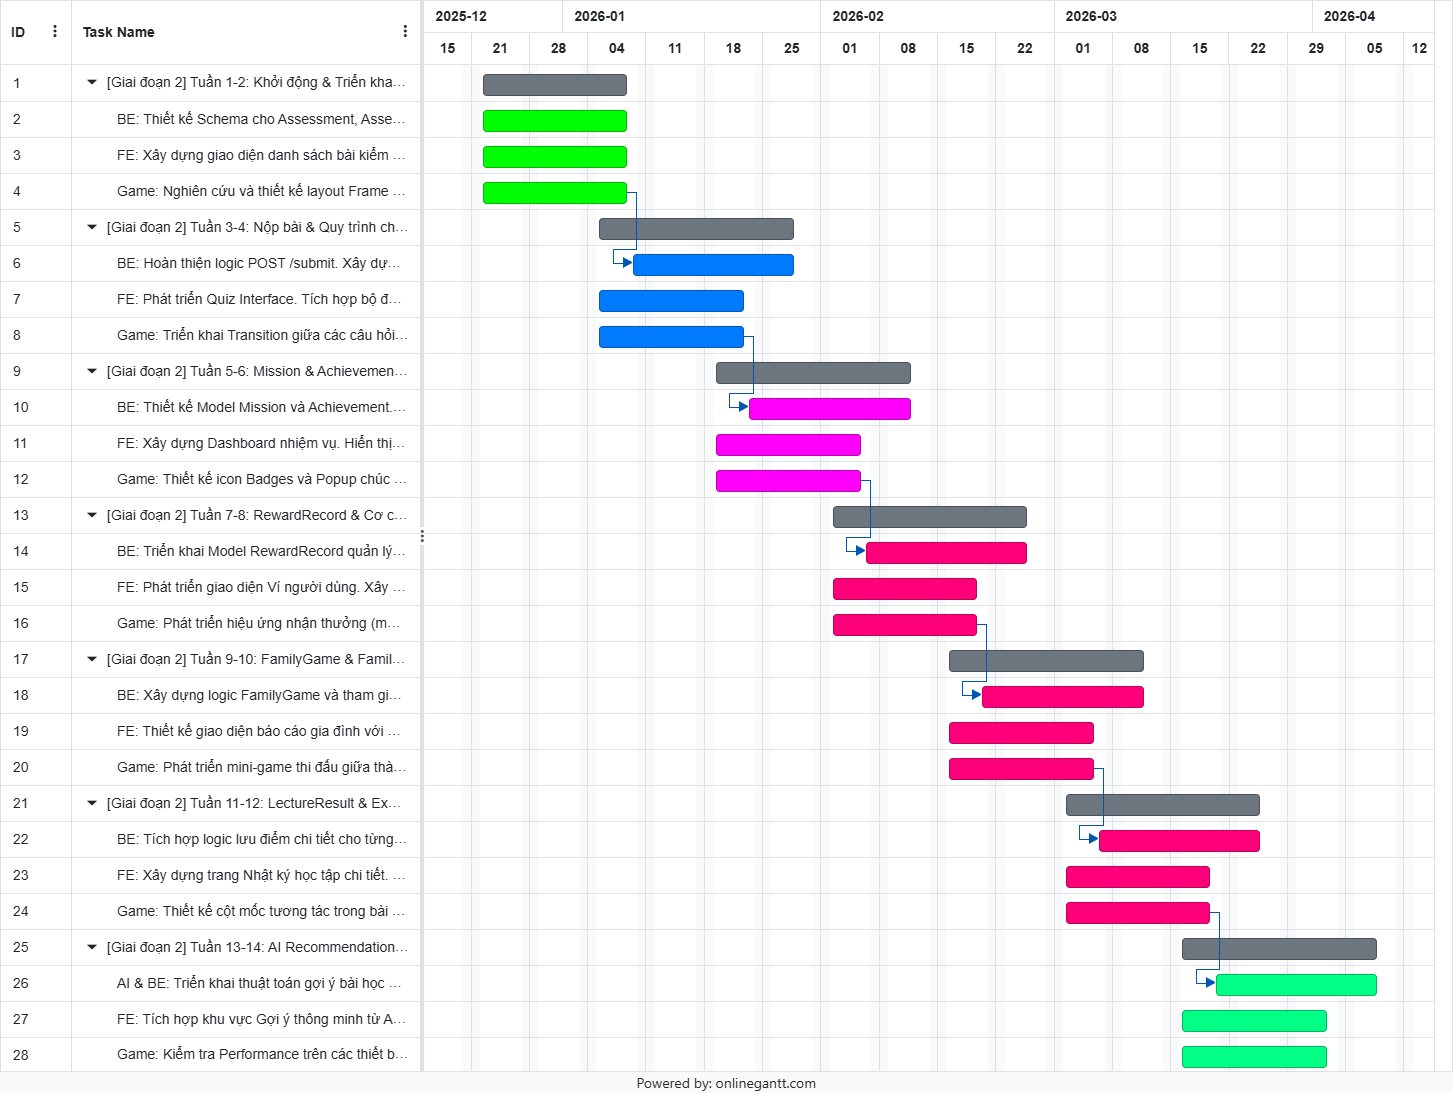
\includegraphics[width=\textwidth]{Image/phase2.jpg}
	\vspace{0.5cm}
	\caption{Biểu đồ Gantt giai đoạn 2}
	\label{fig:gantt-phase2}
\end{figure}

\subsection{Kết quả giai đoạn 2}
Sau khi kết thúc giai đoạn 2, nhóm đã hoàn thiện được các công việc sau đây:
\begin{enumerate}
	\item Hoàn thiện hệ thống bài kiểm tra (Assessment), bao gồm luồng làm bài trực tuyến, bộ đếm ngược thời gian, chấm điểm tự động và hiển thị kết quả.
	\item Hoàn thiện cơ chế nhiệm vụ (Mission) và thành tựu (Achievement), tự động cập nhật tiến trình dựa trên hành động của người dùng.
	\item Hoàn thiện hệ thống phần thưởng (RewardRecord) quản lý lịch sử biến động điểm thưởng của người dùng.
	\item Xây dựng đầy đủ giao diện và chức năng quản trị hệ thống (Admin), bao gồm:
	\begin{itemize}
		\item Quản lý tài khoản người dùng (tìm kiếm, lọc theo vai trò, khóa/mở khóa tài khoản).
		\item Trang thống kê tổng quan hệ thống.
	\end{itemize}
	\item Hiện thực được \textbf{18 dạng toán tương tác} phục vụ học sinh luyện tập bám sát chương trình của Bộ Giáo dục và Đào tạo.
	\item Hiện thực được \textbf{1 minigame} đơn người chơi.
	\item Hiện thực được \textbf{1 game tương tác 2 người} theo thời gian thực.
	\item Lưu trữ chi tiết kết quả học tập (LectureResult, ExerciseResult), hỗ trợ người dùng xem lại lịch sử và các bài tập đã làm sai.
	\item Hoàn thiện báo cáo gia đình (FamilyReport) với các biểu đồ so sánh hiệu suất học tập giữa các thành viên.
\end{enumerate}

\vspace{0.3cm}
\noindent\textbf{Hạn chế còn tồn đọng:} Nhóm chưa hoàn thành được tính năng tích hợp AI để tự động sinh bài tập theo trình độ người dùng. Đây sẽ là hướng phát triển tiếp theo của hệ thống trong tương lai.

